\documentclass{article}
\usepackage{blindtext}
\usepackage{geometry}
\usepackage{array}
\usepackage{graphicx}
\graphicspath{ {./images/} }
 \geometry{
 a4paper,
 total={170mm,257mm},
 left=20mm,
 top=20mm,
 }
\usepackage{amsmath}
\usepackage{hyperref}
\title{writeup of ABC project}

\begin{document}

\maketitle
\section{brief summary}
$\href{https://arxiv.org/abs/1208.2157}{Here is the paper our work is based on.}$ Basically what we are attempting to do is the following:

we have some networks in which hate speech/misinfo have spread. $G^{*}_{T}$ is the network $G^*$, the real network(s) we're studying, at timestamp T.

we have some function $F(G)$ that produces a vector of network characteristics $\phi$.   

our vector of "correct" network characteristics comes from a real network (or many real networks in aggregate) and is denoted as $\phi^*$. 

we have a markovian data generating process that occurs on randomly generated networks of actors. within each experiment, the network model will be the same (e.g. Erdos-Reyni, configuration model, hyperbolic graphs, etc).

during the data generating process $H(\theta, T)$, the network evolves; individual actors may change characteristics, share information, or influence other actors. after $T$ timesteps, the simulation is considered to have concluded, and we have a graph $G_T$.

what is $\theta$? $\theta$ is a parameter vector that governs the distributions from which the actors' characteristics and spreading parameters are drawn. for a toy example, let's say that our actors' susceptibility to misinfo $\mu$ is drawn from a beta distribution $\mu ~ \beta(s_1, s_2)$ and the likelihood of spreading misinfo from one actor to another is $s_3$. $\theta = [s_1, s_2, s_3]$.  

so we have a parameter vector $\theta_i$. we then run our data generation process (network simulation) $H(\theta_i, T)$ for $T$ steps, producing a graph $G_i$. Next, we plug $G_i$ into $F(G)$ to give us $\phi_i$, our vector of network characteristics. 

in order to tell how correct/incorrect our simulation was (compared to $G^*_T$), we compare $\phi_i$ and $\phi^*$ using a "goodness of fit" function / acceptance probability function $Z(\phi_i, \phi^*)$. 

better $\theta_i$ vectors will lead to better values of $\phi_i$; our end goal is to get a distribution over $\theta_i$ vectors. we aren't trying to solve for $\theta_i$; instead, we'd like to know how it's distributed and how much uncertainty we're dealing with.

\section{algorithm}
here's a brief description of the algorithm in the paper, as we understand it.

first, we create a prior on $\theta$. for simplicity's sake (the paper covers this case), we make a uniform prior on $\theta$ while constraining the values to reasonable ranges. for our purposes, we are primarily dealing with beta distributions, so we have a bunch of integer ranges from 1 to 10 that we draw from. future versions of this simulation will also try to infer the Markov steps for agent characteristic updates during the simulation.

next, we draw \textbf{ensemble P} from the prior distribution. \textbf{ensemble P} is a bunch of vectors $\theta^P_i$ that aren't trying to do well. their job is to give us a sense of what the distribution of the badness function $Z(\phi_i, \phi^*)$ is. if \textbf{ensemble P} is large enough, it should give us a good sense of how the badness function values are distributed. we smooth this distribution as well before continuing.

after that, we create \textbf{ensemble E}. the items in \textbf{ensemble E} are "good" compared to the "background" distribution given by the $\theta^P_i$ values in \textbf{ensemble P}. this can take a while because we reject a lot of samples, but is not computationally expensive compared to the rest of the simulation.

we also create a cooling rate parameter $\epsilon_t$ that varies as time goes on. this makes us less likely to make risky jumps in the distribution / make risky decisions when we are further into the process.

now the fun part: we choose a random parameter $\theta^E_i$ in \textbf{ensemble E}. then we generate another $\theta^E_{new}$. we compare the results of $Z(\phi^E_i, \phi^*)$ and $Z(\phi^E_{new}, \phi^*)$ using a "temperature" function $\tau$. $\tau(Z_1, Z_2)$ gives us the probability of keeping $\theta^E_{new}$. then we do a uniform draw and decide whether or not we're keeping $\theta^E_{new}$. if so, $\theta^E_{new}$ becomes the new $i^{th}$ member of \textbf{ensemble E}. 

we do a bunch of iterations of this step, stopping when the rolling acceptance probability of keeping a newly generated sample goes below a certain threshold. 

when we finish our algorithm, \textbf{ensemble E} should give us a sense of how $\theta^*$, the "correct" parameters to produce $\phi^*$, is distributed. for example, here are some heatmaps over the beta distribution parameters for a couple of the agent characteristic distributions. 

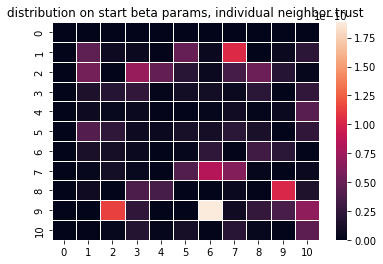
\includegraphics{heatmap_neighbor_trust}
\\
\\
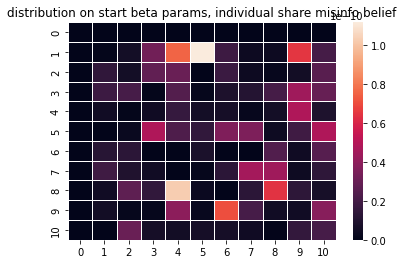
\includegraphics{heatmap_misinfo_belief}
\end{document}
